\documentclass[%
	handout
]{beamer}

\usepackage[utf8]{inputenc}
\usepackage[ngerman]{babel}
\usepackage[T1]{fontenc}

\usepackage{caption}

\usepackage{graphicx}

\usepackage{p4}

%\usetheme[compress]{Dresden}
%\usecolortheme{beaver}


\author{Louis Kobras}
\title{Projektstrukturierungstechniken}
\renewcommand{\date}{08. Juli 2016}

\newcommand{\waterfall}{[Royce1970]}
\newcommand{\waterfallmodel}{[OXAgile]}
\newcommand{\cpm}{[CPM]}
\newcommand{\howtogantt}{[Smartdraw]}
\newcommand{\pmhut}{[PM-Hut]}
\newcommand{\daily}{[AgileDaily]}
\newcommand{\tq}{[Agile3Q]}

\begin{document}

\begin{frame}
	\maketitle
	\vspace{-0.2cm}
	\begin{center}
		Seminar Konzepte verteilter Softwareentwicklung
	\end{center}
\end{frame}

\begin{frame}
	\frametitle{Motivation}
	todo...
\end{frame}

\begin{frame}
	\frametitle{Einführung}
	todo...
\end{frame}

\begin{frame}
	\tableofcontents
\end{frame}

\section{Geschichtlicher Überblick}
	\subsection{Ursprünge im Wasserfall}
		\begin{frame}
			\begin{itemize}
				\item Beginn als Wasserfallmodell\pause
				\item entlehnt aus Ingenieurswesen\pause
				\item nicht sinnvoll für Software anwendbar\pause
			\end{itemize}
			\pause
			\begin{itemize}
				\item 7 Phasen im Original \waterfall\pause, 5 nach Konsolidierung\pause
				\item Code-Schreiben auf 30-40\% reduziert \waterfallmodel\pause
				\item kein guter Umgang mit Änderungen
			\end{itemize}
		\end{frame}
		
		\begin{frame}[fragile]
			\begin{figure}
				\begin{center}
					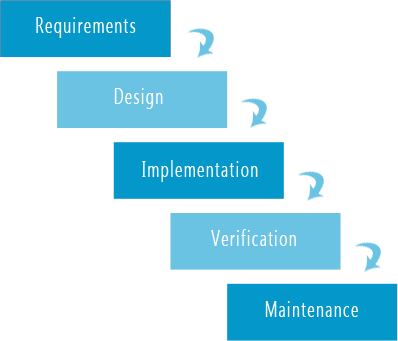
\includegraphics[scale=.5]{../images/waterfall.png}
					\caption{Modifiziertes Wasserfallmodell}
					\label{img:waterfall}
				\end{center}
			\end{figure}
		\end{frame}
	\subsection{Flexible Modelle}
		\begin{frame}
			\begin{itemize}
				\item Anfänge späte 80er frühe 90er\pause
				\item Fokus auf Flexibilität\pause
				\item Ablehnung ``schwergewichtiger'' dokumentationslastiger Softwareentwicklung\pause
				\item Entwicklung von Prototyping, Spiralmodell, Scrum, XP et. al.\pause
				\item ``iterativ'', ``inkrementell'', ``lightweight''
			\end{itemize}
		\end{frame}
	\subsection{Agile Entwicklung}
		\begin{frame}
			\begin{itemize}
				\item Treffen 2001
				\item Festlegung auf gemeinsame Prinzipien
				\item ``Agiles Manifest''
				\item 4 Grundsätze, 12 Prinzipien
				\item unterschrieben von u.A. den Scrum-Entwicklern und den XP-Entwicklern
			\end{itemize}
		\end{frame}
		
		\begin{frame}
			\begin{center}
				Wir erschließen bessere Wege, Software zu entwickeln,\\
				indem wir es selbst tun und anderen dabei helfen.\\
				Durch diese Tätigkeit haben wir diese Werte zu schätzen gelernt:\\
			\end{center}
			\pause
			\begin{itemize}
				\item Individuen und Interaktionen mehr als Prozesse und Werkzeuge
				\item Funktionierende Software mehr als umfassende Dokumentation
				\item Zusammenarbeit mit dem Kunden mehr als Vertragsverhandlung
				\item Reagieren auf Veränderung mehr als das Befolgen eines Plans
			\end{itemize}
			\pause
			\begin{center}
				Das heißt, obwohl wir die Werte auf der rechten Seite wichtig finden,\\
				schätzen wir die Werte auf der linken Seite höher ein.\-\\\-\\
				(\url{http://agilemanifesto.org/iso/de/manifesto.html})
			\end{center}
		\end{frame}
		
\section{Langzeitstrukturierung}
	\subsection{}
		\begin{frame}
			\begin{itemize}
				\item Techniken aus dem Projektmanagement\pause
				\item Überblick über das gesamte Projekt\pause
				\item Engpässe erkennen, Ressourcen verwalten, Deadlines im Auge behalten\pause
			\end{itemize}
		\end{frame}
		
	\subsection{Critical Path}
		\begin{frame}
			\frametitle{Hintergrund}
			\begin{itemize}
				\item Fabrikkonstruktion in den USA 195n
				\item \textit{kritischer Pfad}, ohne den ein Projekt nicht abgeschlossen werden kann
				\item berücksichtigt Abhängigkeiten und Fehlertoleranz
			\end{itemize}
		\end{frame}
		
		\begin{frame}
			\frametitle{Critical Path Analysis (CPA)}
			\begin{enumerate}
				\item Aufgaben nach Abhängigkeiten in Flowchart sortiert\pause
				\item Zeitanforderungen aller Pfade vergleichen\pause
				\item Pfad mit größter Zeitanforderung ist Critical Path\pause
			\end{enumerate}
		\end{frame}
		
		\begin{frame}
			\frametitle{Pro und Contra}
			\begin{minipage}[t]{.48\textwidth}
				Pro:
				\begin{itemize}
					\item erhöht Effizienz und Produktivität
					\item Pfad nimmt Rücksicht auf Störungen\\
						$\Longrightarrow$ Deadlines werden nicht in Mitleidenschaft gezogen
					\item Ressourcenengpässe im Vorraus bekannt
				\end{itemize}
			\end{minipage}
			\begin{minipage}[t]{.48\textwidth}
				Contra:
				\begin{itemize}
					\item kann schnell unübersichtlich werden
					\item Erfüllung kann viel micromanagement erfodern
				\end{itemize}
			\end{minipage}
		\end{frame}
		
		\begin{frame}
			\begin{figure}
				\begin{center}
					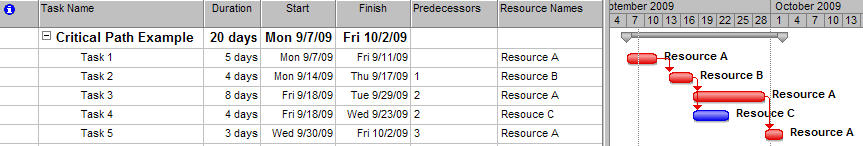
\includegraphics[scale=.5]{../images/critical-path.jpg}
					\caption{Critical Path}
					\label{img:crit}
				\end{center}
			\end{figure}
		\end{frame}
		
	\subsection{PERT}
		\begin{frame}
			\frametitle{Einführung}
			\begin{itemize}
				\item Von der US-Navy für Atom-U-Boote kreiert\pause
				\item Alternative zu CPM mit mehr analytischem Ansatz\pause
				\item Milestones und Aktivitäten statt Tasks
			\end{itemize}
		\end{frame}
		
		\begin{frame}
			\frametitle{Konstruktion}
			\begin{itemize}
				\item Zeit einer Aktivität lässt sich durch Formel approximieren\pause
			\end{itemize}
			\[
				E = \frac{B +4\cdot A+W}{6}
			\]\pause
			\begin{itemize}
				\item Berücksichtigt Extremfälle, legt aber mehr Gewicht auf Normalfall\pause
				\item Anordnen der Milestones und Aktivitäten in Flowchart\pause
				\item Kritischer Pfad aus Diagramm ablesbar
			\end{itemize}
		\end{frame}
		
		\begin{frame}
			\frametitle{Pro und Contra}
			\begin{minipage}[t]{.48\textwidth}
				Pro:
				\begin{itemize}
					\item gibt erwartete Fertigstellungszeit an
					\item Start- und Endzeit von Tasks sind einsehbar
					\item gute Übersicht über Abhängigkeiten
				\end{itemize}
			\end{minipage}
			\begin{minipage}[t]{.48\textwidth}
				Contra:
				\begin{itemize}
					\item Zeitschätzug nach wie vor subjektiv
					\item Lässt weniger \textit{float}, sodass Nebenpfade kritisch werden können
					\item kann ebenfalls schnell unübersichtlich werden
				\end{itemize}
			\end{minipage}
		\end{frame}
		
		\begin{frame}
			\begin{figure}
				\begin{center}
					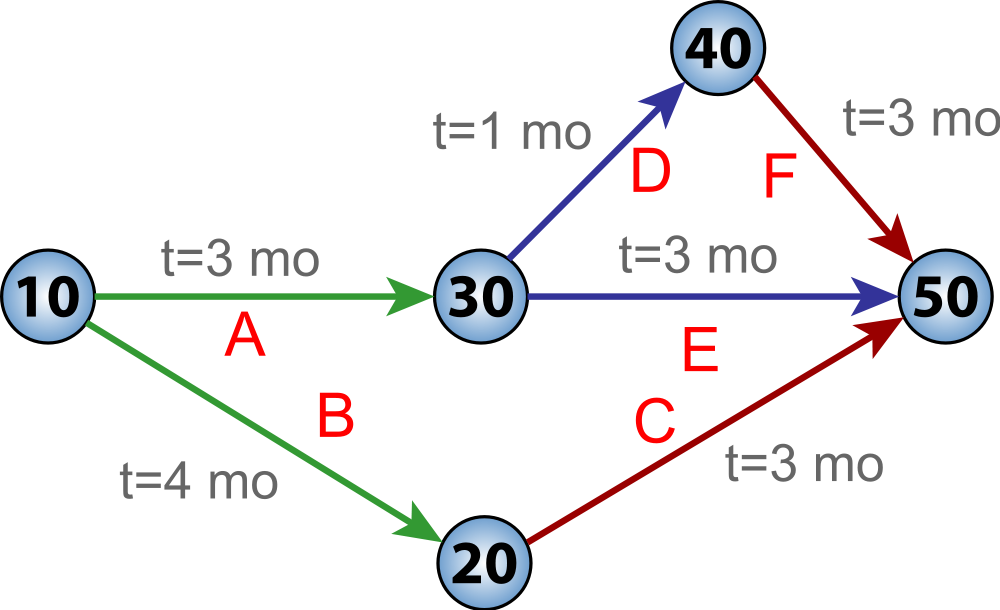
\includegraphics[scale=.2]{../images/pert.png}
					\caption{PERT-Diagramm}
					\label{img:pert}
				\end{center}
			\end{figure}
		\end{frame}
		
	\subsection{Gantt-Diagramme}
		\begin{frame}
			\frametitle{Einführung}
			\begin{itemize}
				\item Offiziell 191n von Henry Gantt entwickelt \pause
				\item ähnliches System 1896 von Karol Adamiecki verwendet, allerdings erst 1931 veröffentlicht\pause
				\item stellt Zeiten im Projekt dar\pause, moderne Darstellungen stellen auch Abhängigkeiten dar\pause
				\item unterstützt PERT und CPM
			\end{itemize}
		\end{frame}
		
		\begin{frame}
			\frametitle{Konstruktion}
			\begin{itemize}
				\item Ziele des Projektes klar definieren\pause
				\item Aufgaben nach Verfügbarkeit und Fähigkeit der Teammitglieder verteilen\pause
				\item Task-Dauer bestimmen (PERT-Formel)\pause
				\item Abhängigkeiten auflösen (CPM)\pause
				\item Diagramm mit Team abstimmen \howtogantt
			\end{itemize}
		\end{frame}
		
		\begin{frame}
			\frametitle{Pro und Contra}
			\begin{minipage}[t]{.48\textwidth}
				Pro:
				\begin{itemize}
					\item Sortieren von Projektdetails
					\item einfaches Darstellen komplexer Zusammenhänge
					\item unterstützt bei Erstellung,Einhaltung und Überarbeitung von Deadlines
					\item Außenstehende erhalten leicht einen Überblick \pmhut
				\end{itemize}
			\end{minipage}
			\begin{minipage}[t]{.48\textwidth}
				Contra:
				\begin{itemize}
					\item sehr schnell enorme Ausmaße
					\item muss stets aktuell gehalten werden
					\item Hang zur Unübersichtlichkeit
				\end{itemize}
			\end{minipage}
		\end{frame}
		
		\begin{frame}
			\begin{figure}
				\begin{center}
					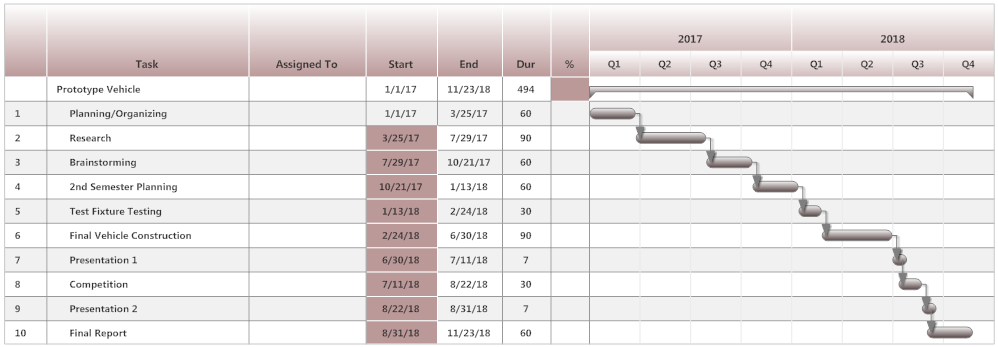
\includegraphics[scale=.1]{../images/gantt2.png}
					\caption{Ein Gantt-Diagramm mit Critical Path}
					\label{img:gantt}
				\end{center}
			\end{figure}
		\end{frame}
		
\section{Kurzzeitstrukturierung}
	\subsection{}
		\begin{frame}
			\begin{itemize}
				\item Techniken aus Softwareentwicklungspraktiken
				\item entnommen aus Lean und Scrum/XP
				\item geeignet für Iterationsmanagement
				\item ungeeignet für Vollständigkeit großer Projekte
			\end{itemize}
		\end{frame}

	\subsection{Kanban}
		\begin{frame}
			\frametitle{Einführung}
			\begin{itemize}
				\item Entnommen aus Lean
				\item Technik zur Autofertigung
				\item beschleunigt und vereinfacht Produktion
				\item justierbar für persönliche Vorlieben(?)
			\end{itemize}
		\end{frame}
		
		\begin{frame}
			\frametitle{Verwendung}
			\begin{itemize}
				\item Auswahl von sinnvollen Kategorien (Backlog, Todo, Doing, Revision, Finished)
				\item Tasks in die entsprechenden Kategorien hängen
				\item zu Beginn jeder Iteration Tasks in die nächste Kategorie hängen
				\item optional: auf WIP-Limit achten
			\end{itemize}
		\end{frame}
		
		\begin{frame}
			\frametitle{Pro und Contra}
			todo...
		\end{frame}
		
		\begin{frame}
			\begin{figure}[h]
				\begin{center}
					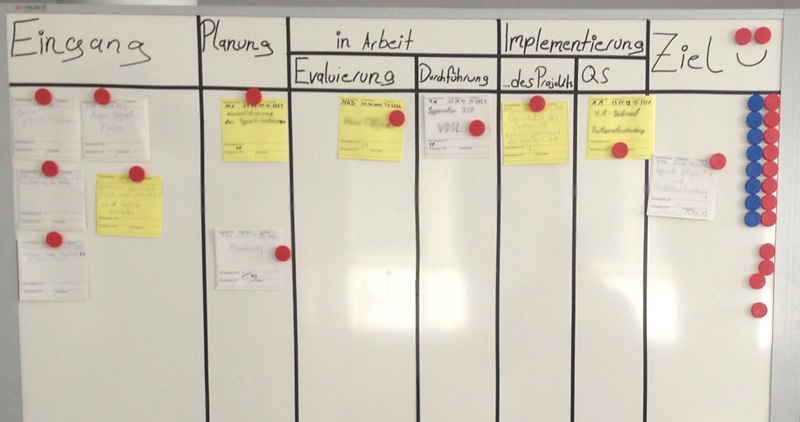
\includegraphics[scale=.3]{../images/kanban-board.jpg}
					\caption{Ein Kanban-Brett}
					\label{img:kanban}
				\end{center}
			\end{figure}
		\end{frame}
		
		\begin{frame}
			\href{http://www.kanbansim.org/boards/3a5a5acdb1c24535e9962dd20fe434b3}{Live-Beispiel}
		\end{frame}
		
	\subsection{Daily Scrum und Stand-Up-Meeting}
		\begin{frame}
			\frametitle{Einführung}
			\begin{itemize}
				\item Technik aus Scrum und XP\pause
				\item täglich zur gleichen Zeit am gleichen Ort\pause
				\item entstanden im Scrum 1997, übernommen von XP 1998, als agile Kernpraxis übernommen 2005 \daily\pause
				\item Als Orientierung die 3 Scrum-Fragen \tq
				\begin{enumerate}
					\item Was wurde seit dem letzten Treffen fertig gestellt?
					\item Was soll bis zum nächsten Treffen fertig sein?
					\item Welche Probleme sind aufgetreten?
				\end{enumerate}\pause
				\item sollte nicht länger als 15 Minuten dauern\pause
				\item wird seit XP im Stehen abgehalten
			\end{itemize}
		\end{frame}
		
		\begin{frame}
			\frametitle{Vorteile}
			\begin{itemize}
				\item alle wissen alles wichtige
				\item jeder hat einen Projektüberblick
				\item soziale Vernetzung
				\item weiche Kontrolle über den Projektstatus
			\end{itemize}
		\end{frame}
		
		\begin{frame}
			\frametitle{Probleme}
			\begin{itemize}
				\item ``Scrum-Zombie''-ness
				\item Meeting wird zum Statusbericht
				\item Überlänge
			\end{itemize}
		\end{frame}
		
\section{}
	\subsection{}
		\begin{frame}
			\frametitle{Zusammenfassung}
			todo...
		\end{frame}
		\begin{frame}
			\frametitle{Fazit}
			todo...
		\end{frame}
		\begin{frame}
			\frametitle{Grafikenverzeichnis}
			\begin{tabular}{r|p{.85\textwidth}}
				\textbf{Nummer}		&	\textbf{Quelle}	\\ \hline
		
				\ref{img:waterfall}	&	\textbf{Grafik:} \url{http://www.oxagile.com/wp-content/uploads/2014/02/waterfall.png},
										\textbf{Seite:} \url{http://www.oxagile.com/company/blog/the-waterfall-model/}	\\\hline
				\ref{img:crit}		&	\textbf{Grafik:} \url{http://tr1.cbsistatic.com/hub/i/2009/09/09/76bb5c08-c3b4-11e2-bc00-02911874f8c8/cpm1.jpg},
										\textbf{Seite:} \url{http://www.techrepublic.com/blog/tech-decision-maker/why-critical-path-is-critical-to-project-management/}
			\end{tabular}
		\end{frame}
		\begin{frame}
			\begin{tabular}{r|p{.85\textwidth}}
				\textbf{Nummer}		&	\textbf{Quelle}	\\ \hline
				\ref{img:pert}		&	\textbf{Grafik:} \url{https://upload.wikimedia.org/wikipedia/commons/thumb/3/37/Pert_chart_colored.svg/1000px-Pert_chart_colored.svg.png},
										\textbf{Seite:}	 \url{https://en.wikipedia.org/wiki/Program_evaluation_and_review_technique}\\\hline
				\ref{img:gantt}		&	\textbf{Grafik:} \url{https://wcs.smartdraw.com/cmsstorage/exampleimages/49d69987-97a4-4d57-8123-262e16a32261.png?bn=1510011143},
										\textbf{Seite:} \url{https://www.smartdraw.com/gantt-chart/examples/prototype-vehicle-gantt-chart/}
			\end{tabular}
		\end{frame}
		\begin{frame}
			\begin{tabular}{r|p{.85\textwidth}}
				\textbf{Nummer}		&	\textbf{Quelle}	\\ \hline
				\ref{img:kanban}	&	\textbf{Grafik:} \url{http://blog.novatec-gmbh.de/wp-content/uploads/2013/05/kanban-board.jpg}, 
		
			\end{tabular}
		\end{frame}
		\begin{frame}
			\frametitle{Quellenverzeichnis}
			todo...
		\end{frame}
	
\end{document}